\documentclass{prova}

\usepackage{amssymb}
\usepackage[inline]{enumitem}

\newcommand{\sen}{\,\mbox{sen}\,}
\newcommand{\tg}{\,\mbox{tg}\,}
\newcommand{\cosec}{\,\mbox{cosec}\,}
\newcommand{\cotg}{\,\mbox{cotg}\,}
\newcommand{\tr}{\,\mbox{tr}\,}
\newcommand{\ds}{\displaystyle}
\newcommand{\ra}{\rightarrow}

\professor{Prof.\@ Adriano Barbosa}
\disciplina{C\'alculo Diferencial e Integral}
\avaliacao{PS}
\curso{Engenharia de Produção}
\data{01/06/2021}

\begin{document}
	\cabecalho{5}  % o numero 5 indica a qnt de quadros na tabela de nota

	\textbf{Todas as respostas devem ser justificadas.}

    \vspace{0.5cm}

    {\bf Avalia\c{c}\~ao P1:}
	\begin{questionario}
        \q{Determine se as afirmações são verdadeiras ou falses justificando sua resposta:}
            \begin{questionario}
                \qq{(1 pt) Se $f$ é contínua em $[a,b]$, então $f$ é derivável em $(a,b)$.}
                \qq{(1 pt) Se $f(x) = \sqrt{x}$ e $g(x) = x^2-1$, então $h(x) = (g\circ f)(x)$
                    pode ser calculada para todo $x\in\mathbb{R}.$}
                \qq{(1 pt) Se $f(0)>0$ e $f(1)<0$, então existe um número $c$
                    entre $0$ e $1$ tal que $f(c)=0$.}
            \end{questionario}
        \q{(2 pt) Se $2x-\frac{1}{2}\leqslant f(x)\leqslant 2x^2$ para $0<x<1$,
            calcule $\ds \lim_{x\rightarrow \frac{1}{2}}f(x)$.}
        \q{(2 pt) Mostre que a equação $3\cos{x} = 1-3x^3$ tem uma solução no intervalo $[-1, 1]$.}
        \q{Seja $s(t)=-2t^3+10t^2$ a função que descreve a posição de um móvel em função do tempo.}
            \begin{questionario}
                \qq{(0,5 pt) Qual a função velocidade do móvel?}
                \qq{(1 pt) Em $x=2$ o móvel está movendo-se para frente ou para trás?}
                \qq{(0,5 pt) Em quais instantes de tempo a velocidade é nula?}
                \qq{(1 pt) Sabendo que a aceleração é a taxa de variação da
                    velocidade, podemos dizer que a aceleração é constante? Por
                    quê?}
            \end{questionario}
	\end{questionario}

    \vspace{1cm}

    {\bf Avalia\c{c}\~ao P2:}
    \begin{questionario}
        \q{(2,0 pt) Uma escada de 10 metros está encostada numa parede e seu pé desliza
            a uma taxa de 1m/s. Quão rápido o ângulo entre a escada e o chão
            está variando quando o pé da escada estiver a 6 metros da parede.}
        \q{(2,5 pt) Quais devem ser as dimensões de um cartaz regantular de modo que
            sua área impressa seja 192~cm$^2$, que as margens superior e inferior 
            tenham 3 cm cada, que as margens laterais tenham 2 cm cada e seja
            utilizado a menor quantidade possível de papel para sua fabricação?}
        \q{(2,5 pt) Mostre que 4 é um número crítico da função $f(x)=(x-4)^3 - 1$ e que
            $f$ não tem máximo ou mínimo local em 4.}
        \q{Seja $g(x)=\ds\int_0^x f(t)\ dt$, onde o gráfico de $f$ é dado abaixo:}
            \begin{figure}[h]
                \centering
                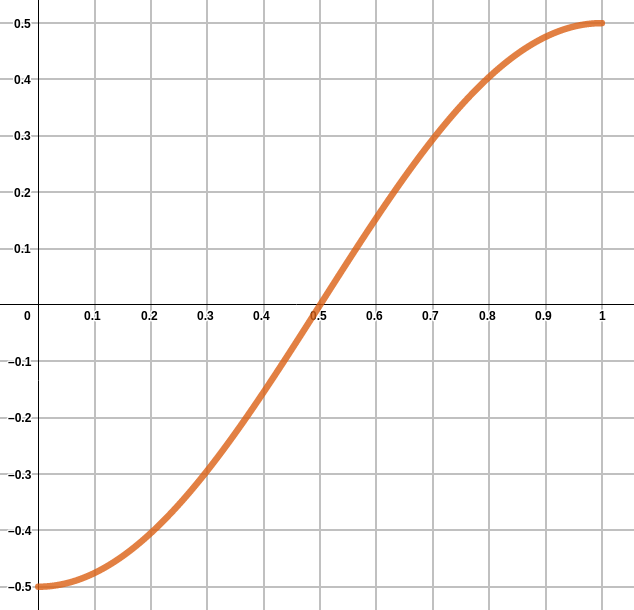
\includegraphics[width=0.4\textwidth]{grafico.png}
            \end{figure}
            \begin{questionario}
                \qq{(0,5 pt) Calcule $g(0)$ e $g(1)$. Justifique sua resposta.}
                \qq{(0,5 pt) Estime o valor de $g(0,1)$}
                \qq{(1 pt) Em qual intervalo $g$ é crescente?}
                \qq{(1 pt) Onde $g$ possui valor máximo ou mínimo? Onde?}
            \end{questionario}
    \end{questionario}
\end{document}
